%%%%%%%%%%%%%%%%%%%%%%%%%%%%%%%%%%%%%%%%%%%%%%%%%%%%%%%%%%%%%%%%%%%
\section{Étape 5: Portage et optimisation du code} \label{sec:methodo_step5}
%%%%%%%%%%%%%%%%%%%%%%%%%%%%%%%%%%%%%%%%%%%%%%%%%%%%%%%%%%%%%%%%%%%

Lors de l'étape 4, une plateforme a été choisie en fonction de plusieurs critère pour y porter les noyaux. L'étape 5 s'occupe du portage du code et de la validation du modèle de performance. 


%%%%%%%%%%%%%%%%%
\subsection{Introduction}
%%%%%%%%%%%%%%%%%

    \subsubsection{Motivations}
    %%%%%%%%%%%%%%%%%%%%%%%%%%%%%%
    Une fois le choix de la plateforme adaptée au noyau dans l'étape 4, le travail de portage doit être réalisé. 
    Une difficulté rencontrée par le programmeur est de s'assurer que les performances obtenues après le portage sont celles attendues par les prédictions. L'utilisation d'une nouvelle plateforme apporte une difficulté supplémentaire concernant la compatibilité des outils. Le programmeur doit alors être capable de poursuivre son analyse de performance avec des outils simples. 
    L'objectif de cette étape est de montrer au programmeur comment les outils présentés dans cette thèse, peuvent l'aider à valider la performance du noyau établie lors de l'étape 3.

    
    \subsubsection{Premier développement}
    %%%%%%%%%%%%%%%%%
        Une fois la plateforme choisie il faut appliquer les transformations du code nécessaires pour pouvoir y exécuter les noyaux. L'effort nécessaire pour adapter le code à cette nouvelle architecture a dû être évalué lors de l'étape précédente. Le portage du code peut nécessiter un changement de langage de programmation ou de paradigme de programmation.
        Si possible, il est important d'utiliser des librairies déjà optimisées pour espérer atteindre les performances crêtes de l'application. De plus, les constructeurs de la plateforme peuvent avoir développé des librairies pouvant être quasi-optimales et qui nécessitent une grande expertise pour être développées.
        
        Pour atteindre le maximum de performance, le code doit profiter au maximum de la parallélisation. Pour cela, le maximum de coeurs doivent être utilisés, grâce aux paradigmes de programmation partagée et distribuée. Les processeurs étant généralement superscalaires (voir \autoref{sec:superscalar}) il faut essayer d'exécuter le maximum d'instructions chaque cycle. Le dernier niveau de parallélisme est apporté par l'utilisation d'instructions vectorielles. Lorsque c'est possible des instructions telles que les FMA doivent être utilisées. Les différentes pistes listées peuvent nécessiter l'utilisation d'un simple drapeau lors de la compilation ou au contraire nécessiter de lourdes modifications du code et des jeux de données.
    

\subsection{Analyse de performance}
%%%%%%%%%%%%%%%%%

    Lors de l'étape 4, un modèle de performance du noyau a été établi (voir paragraphe \ref{sec:smm}). Une fois porté sur la nouvelle plateforme, il convient de vérifier les performances obtenues. La \autoref{pic:methodo_step5} propose un cheminement à suivre pour la validation et l'optimisation des performances.

\begin{figure}[h!]
    \center
    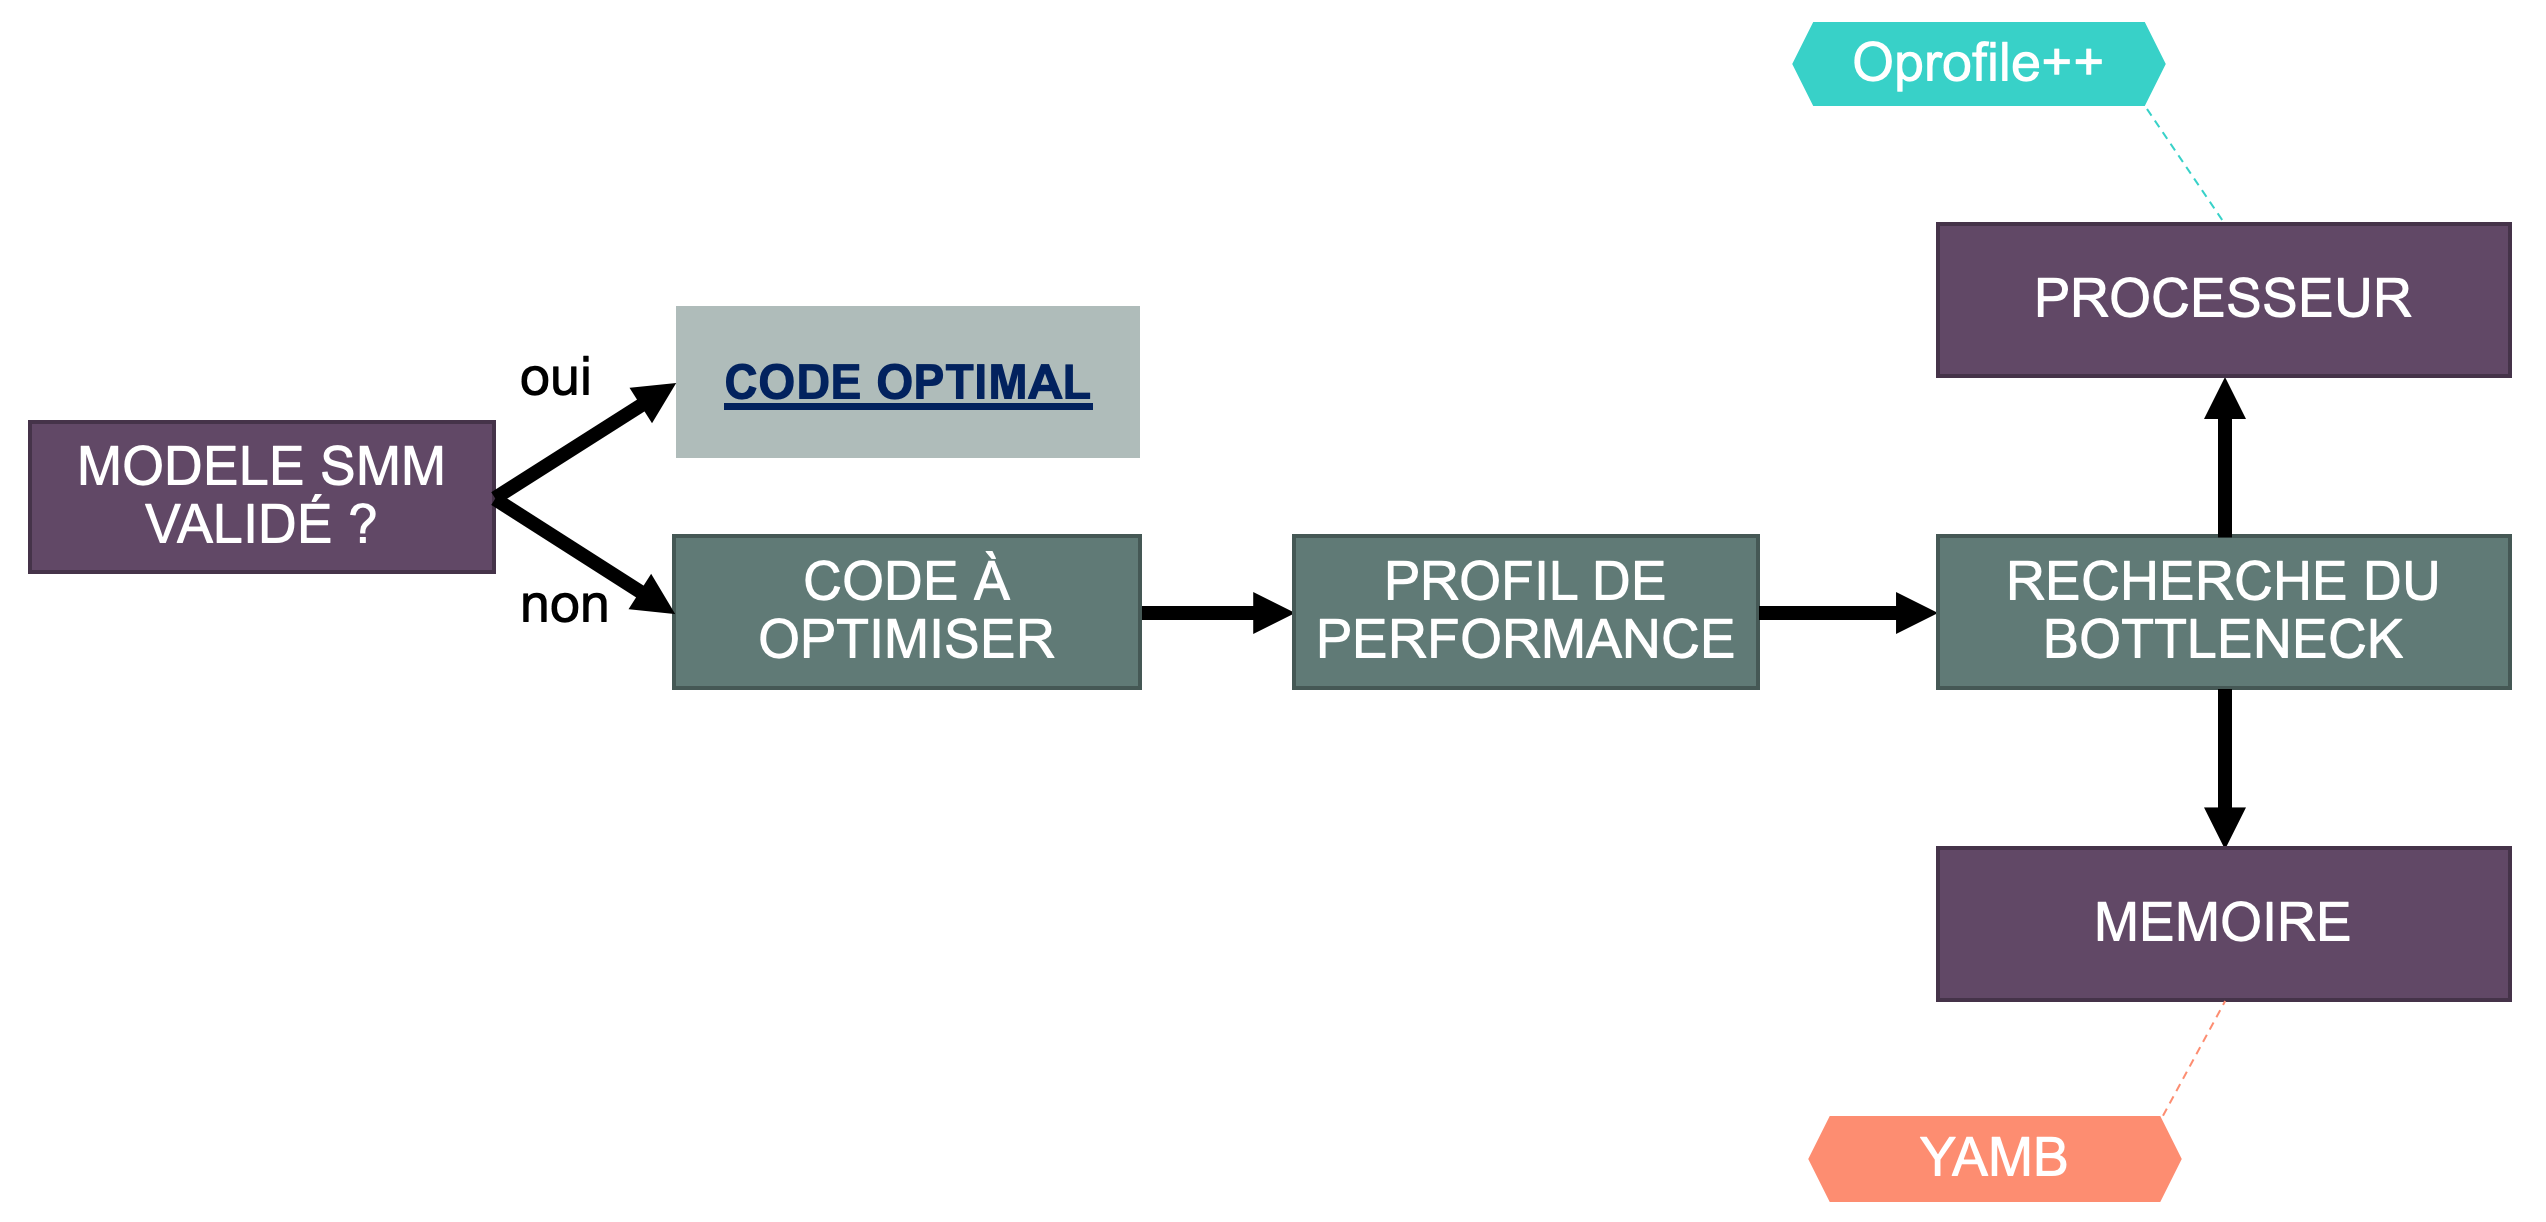
\includegraphics[width=14cm]{images/methodo_step5.png}
    \caption{\label{pic:methodo_step5}Les différentes étapes à suivre pour valider la performance du noyau.}
\end{figure}




    \subsubsection{Vérification du modèle de performance}
    %%%%%%%%%%%%%%%%%
    
        La première étape de l'analyse est de valider que la performance atteinte par le code est proche de celle calculée par notre modèle SMM. Dans le cas contraire, cela permet de quantifier l'écart par rapport à l'optimum théorique $\text{TEMPS}_{optimal}$. 
        
        Pour mesurer le temps d'exécution du noyau, $\text{TEMPS}_{mesure}$, nous proposons d'utiliser la fonction \textit{gettimeofday ()} \cite{Linux}. Cette fonction est disponible sur la totalité des systèmes Linux et permet de récupérer l'heure actuelle avec une précision allant jusqu'à la microseconde. Le but de la méthodologie présentée est de porter les codes sur de nouvelles architectures. Baser l'analyse de performance sur des compteurs matériels trop complexes aurait réduit la portabilité de notre démarche. On peut mesurer  $\text{TEMPS}_{mesure}$ en plaçant deux appels à la fonction \textit{gettime} présentée dans l'\autoref{lst:gettime}, avant et après le noyau.
        
        
        \begin{lstlisting}[language=c,caption=Fonction utilisée pour lire la date actuelle avec une précision allant jusqu'à la microseconde,label={lst:gettime}, 
          basicstyle=\footnotesize, frame=tb,
          xleftmargin=.065\textwidth, xrightmargin=.065\textwidth]
        double gettime()
        {
          struct timeval tp;
          struct timezone tzp;
          int i;
          i = gettimeofday(&tp,&tzp);
          return ( (double) tp.tv_sec + (double) tp.tv_usec * 1.e-6 );
        }
        \end{lstlisting}
        
        Si $\text{TEMPS}_{mesure}$ est proche de $\text{TEMPS}_{optimal}$ alors le noyau est proche d'avoir des performances optimales. Dans le cas contraire, l'analyse de performance doit se poursuivre pour en connaître la cause. La mesure $\text{TEMPS}_{optimal}$ permet d'avoir un objectif de performances à atteindre et de savoir quand le travail d'optimisation est terminé.
        
    
    \subsubsection{Profilage des performances}
    %%%%%%%%%%%%%%%%%

        Si la mesure de $\text{TEMPS}_{mesure}$ est inférieur à l'optimale $\text{TEMPS}_{optimal}$ et que l'optimisation du noyau est envisagée il est alors nécessaire d'en comprendre la raison. Pour cela, le programmeur doit avoir des outils à sa disposition lui permettant mener l'analyse. Même si l'analyse par le modèle du \textit{Roofline} a montré que la performance maximale atteignable était limitée par la bande passante mémoire, d'autres facteurs peuvent affecter les performances (mauvaise compilation, dépendances de données, mauvaise utilisation de la localité). Utilisés de façon méthodique les deux outils présentés dans cette thèse, \textit{OProfile++} et \textit{YAMB}, permettent de répondre à beaucoup de questions et mener à bien le travail d'optimisation du code dont une vue d'ensemble est proposée sur la \autoref{pic:analyse_bigpicture}.
        
        \begin{figure}
            \center
            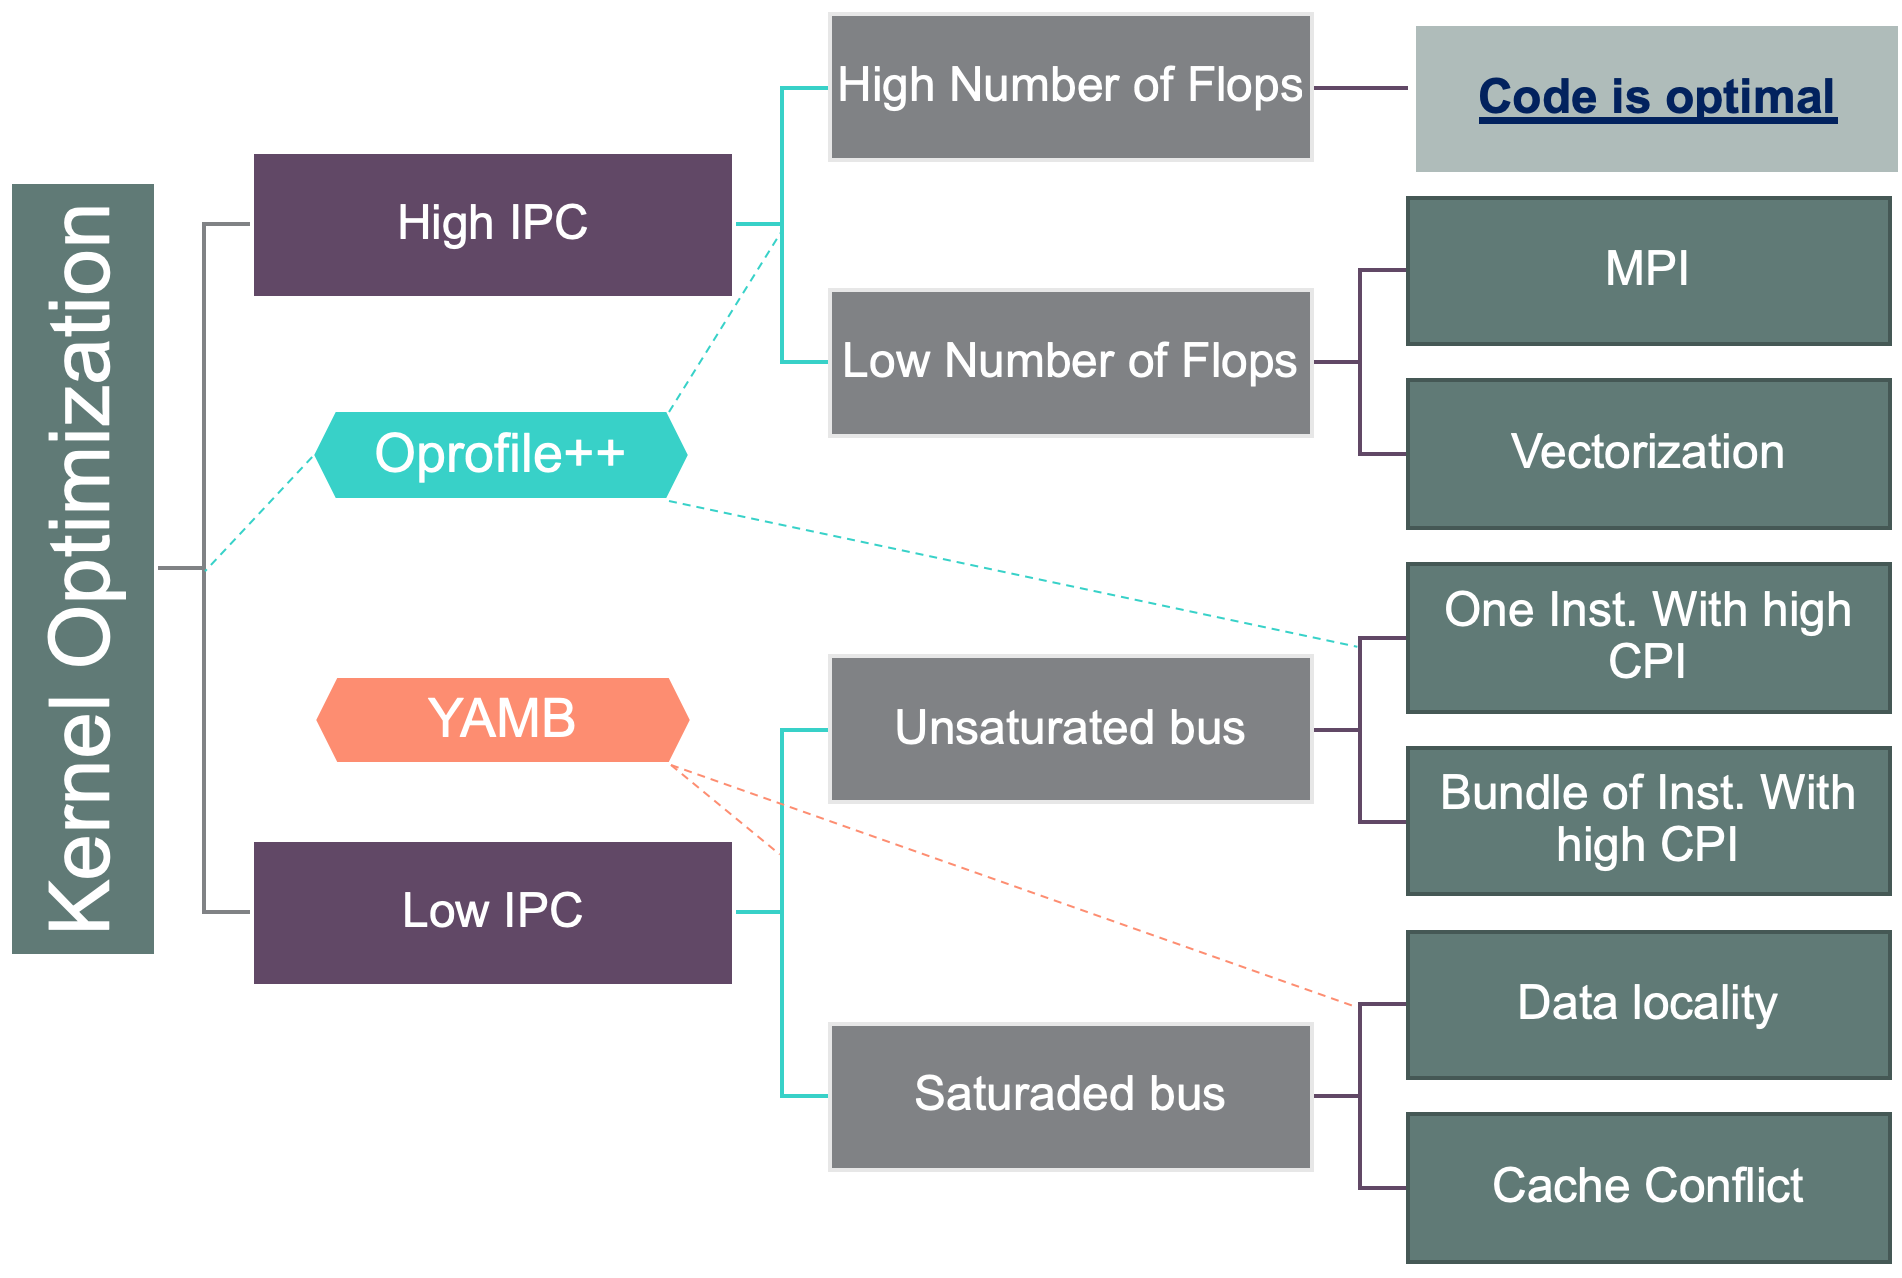
\includegraphics[width=12cm]{images/analyse_bigpicture.png}
            \caption{\label{pic:analyse_bigpicture} Flux de travail pour l'utilisation des outils \textit{Oprofile++} et \textit{YAMB}. En fonction des observations amenées par les outils, des réponses différentes sont proposées au programmeur pour optimiser son code.}
        \end{figure}

        La première mesure à réaliser est celle de l'IPC des boucles critiques du noyau. Pour ce faire, nous avons présenté l'outil \verb=Oprofile++= dans la \autoref{sec:oprofile} (voir \autoref{lst:oprofileex}). Si l'outil indique un IPC faible, il y a de fortes chances que le système mémoire soit responsable de la mauvaise performance. Un IPC élevé indique quand à lui que le problème vient du processeur.
        
        \begin{lstlisting}[language={},caption=L'outil \textit{Oprofile++} permet d'extraire le code assembleur et d'y associer le compteur de cycles,label={lst:oprofileex}, 
  frame=tb]
================================================================
Analysis from the app name (horner1_long) hot spot from the symbole name (f1(double)) which takes 50.1878% 
================================================================
CYCLES       INSTS      ADDRESS    disassembly
----------------------------------------------------------------
     5           11      401be0    vmovupd 0xd1b8(%rip),%ymm1
    39           79      401bf0    vfnmadd231pd 0xd1c7(%rip),%ymm11,%ymm1
     3           14      401bf9    vfmadd213pd %ymm2,%ymm11,%ymm1
...
   760         1652      401c3e    cmp    %eax,%edx
    48           99      401c40    jb     401be0 <_Z8range_f1ddi+0xa0>
----------------------------------------------------------------
LOOP from 401c40 to 401be0  size= 96 sum(cycles)= 2287 
     IPC= 2.12462 cycles/LOOP= 10.3548 flop/cycle = 1.42 
----------------------------------------------------------------
\end{lstlisting}

        
        \subsubsection{Profilage de la mémoire}
        %%%%%%%%%%%%%%%%%
            Lorsque la première analyse indique que la mauvaise performance du noyau est dûe au système mémoire il est nécessaire de réaliser l'analyse de son activité. La première vérification à faire et de s'assurer que le bus mémoire est saturé. Pour y répondre, nous proposons d'utiliser l'outil YAMB (voir \autoref{sec:yamb}) qui affiche l'activité du bus mémoire (lecture, écriture et utilisation totale). Pour confirmer sa saturation, il est nécessaire d'avoir caractérisé la performance du bus mémoire lors de la première étape et d'en connaître la performance maximale. 
            
            Pour valider sa saturation, il est important de posséder une fréquence d'échantillonage suffisamment élevée. En effet, avec une fréquence trop faible, il peut arriver que le graphique montre une saturation avec une ligne droite atteignant la performance maximale. En augmentant le fréquence et en grossissant certaines parties du graphique, il est possible de voir que le bus n'est pas totalement utilisé pendant des périodes très courtes, et saturé quelques cycles après. Ce phénomène peut être dû à des dépendances entres plusieurs instructions. Des techniques de déroulement de boucles sont alors très efficaces si la nature de l'application le permet (voir \autoref{sec:dml_unroll}). Un autre facteur peut venir de la mauvaise gestion du préchargement des données. Il peut alors être intéressant de réaliser le préchargement manuellement en démarrant les chargement de données plusieurs instructions avant qu'elles soient utilisées. D'autres techniques, telles que la fusion de différentes boucles (ou noyau) nous ont permis d'améliorer la performance de plusieurs applications.
            
            Si le bus est bien saturé, nous utilisons le modèle SMM pour comparer les ratio de lecture/écriture avec celui calculé dans l'étape 1 (voir \autoref{sec:smm}). Un mauvais ratio peut provenir d'un nombre de lectures plus élevé que prévu. En effet, il est très rare de réaliser plus d'écriture que nécessaire. Ceci est causé par un large éventail de problèmes potentiels, par exemple, des conflits dans le cache, la lecture de données inutiles, une décomposition incorrecte des données ou des structures de mémoire inappropriées. Pour y remédier, des techniques de \textit{blocking} peuvent être utilisées pour améliorer l'utilisation de la localité des données.  L'outil aide pour trouver si des groupes d'instructions sont plus long à exécuter que d'autres, pouvant être expliqué par une dépendance entre les données ou une donnée non présente dans la mémoire cache au moment requis. 
        
        
        
        \subsubsection{Profilage du processeur}
        %%%%%%%%%%%%%%%%%
        
            Si la première analyse montrait que la mauvaise performance n'était pas dû au système mémoire, il faut alors affiner l'analyse de l'exécution du code donnée par \verb=Oprofile++= (voir \autoref{lst:oprofileex}).
            La première vérification à faire est de compter le nombre d'opérations flottantes réalisées par la boucle. Pour cela, nous comptons manuellement le nombre d'opérations flottantes à partir des instructions assembleurs utilisées. Si le nombre d'opérations flottantes et l'IPC sont élevés, cela indique que le code est optimal. 
            
            Un nombre d'opérations flottantes faible associé à un IPC élevé indiquent que la parallélisation n'est pas correctement utilisée. Il est alors conseillé de regarder le type d'instructions exécutées.
                Un compilateur de mauvaise qualité aura tendance à générer de nombreuses instructions supplémentaires simple à exécuter. Cela fait augmenter l'IPC de la boucle sans en améliorer la performance. Un mauvais compilateur aura tendance à générer plus d'instructions qu'un bon compilateur pour le calcul d'adressage par exemple. La performance du code peut alors être limitée par l'unité de calcul d'adresses et non par la FPU.
                Un autre exemple couramment rencontré est l'exécution d'instructions de la librairie MPI utilisée pour synchroniser les processus. Celles-ci sont exécutées à chaque cycle pour vérifier l'état des autres processus, faisant augmenter l'IPC de la boucle. Il faut alors utiliser des outils tels que Paraver, Extrae ou Vampire pour vérifier que la répartition du travail est bien réalisée. Un noeud de calcul ayant un matériel défectueux affectent alors les autres serveurs, et de nombreux cycles sont perdus dans ces instructions de synchronisation. Les pannes sont très difficiles à identifier sans les outils adaptés car ils peuvent venir d'une mutlitude d'endroits: barette mémoire défectueuse, surchauffe du processeur ou un disque cassé.
                Si la boucle contient beaucoup d'instructions de calculs flottantes, il faut vérifier qu'il s'agit d'instructions vectorielles les plus larges possibles.
            
            Il est donc important de ne pas baser son analyse que sur la lecture de l'IPC mais de vérifier que les instructions exécutées sont des instructions de calculs flottants. Les transformations du code nécessaires pour y parvenir peuvent être difficile à réaliser et demander l'utilisation d'un autre algorithmes ou de restructurer le jeu de données.
            


%%%%%%%%%%%%%%%%%
\subsection{Application au benchmark \textit{Stream}}
%%%%%%%%%%%%%%%%%

    Nous appliquons notre méthodologie sur le benchmark Stream fonctionnant sur un processeur Intel Skylake. Cet exercice nous permet de montrer que même sur un code aussi simple, apparemment optimal, notre analyse nous permet de comprendre sa performance et de l'optimiser.
    
        
    \subsubsection{Vérification du modèle SMM}
    %%%%%%%%%%%%%%%%%
    
        Nous avons montré précédemment que la performance du noyau était limitée par la bande passante mémoire. Nous avons appliqué notre modèle de performance SMM et déterminé $\text{TEMPS}_{optimal}$ égale à $\frac{58.8}{128} = 0.56$ seconde. En utilisant la fonction présenté dans l'\autoref{lst:gettime} nous mesurons $\text{TEMPS}_{mesure} = 0.79$ seconde.
        L'application n'est donc pas optimale. Ceci est également validé par le résultat du benchmark Stream qui annonce une bande passante mémoire de 80,13 GB/sec (à l'aide de \verb=DML_MEM= nous avions mesuré $\text{MEMORY}_{max} = 105 GB/s$).
        
        Pour comprendre ce résultat, nous avons utilisé YAMB pour vérifier que le bus mémoire était bien saturé. Le graphique de la \autoref{fig:stream_before} nous montre que le bus mémoire est utilisé au maximum de son potentiel de 104 GB/s. La saturation du bus n'est donc pas la cause de la mauvaise performance du noyau. Il est alors nécessaire de regarder les rapports lecture/écriture. Lors de l'étape 3, nous avions calculé un ratio optimale pour ce noyau  d'une écriture pour deux lectures. La \autoref{fig:stream_before} montre la répartition mesurée lors de l'exécution: 26 GB/s en écriture pour 78 GB/s en lecture, pour un total de 104 GB/s, ce qui correspond à un ratio de 1 écriture pour 3 lectures. Ce ratio exact d'une écriture pour trois lectures n'est pas une coïncidence. Un vecteur entier est lu alors qu'il ne devrait pas l'être.
        
        \begin{figure}[htb]
        {
        \centering
        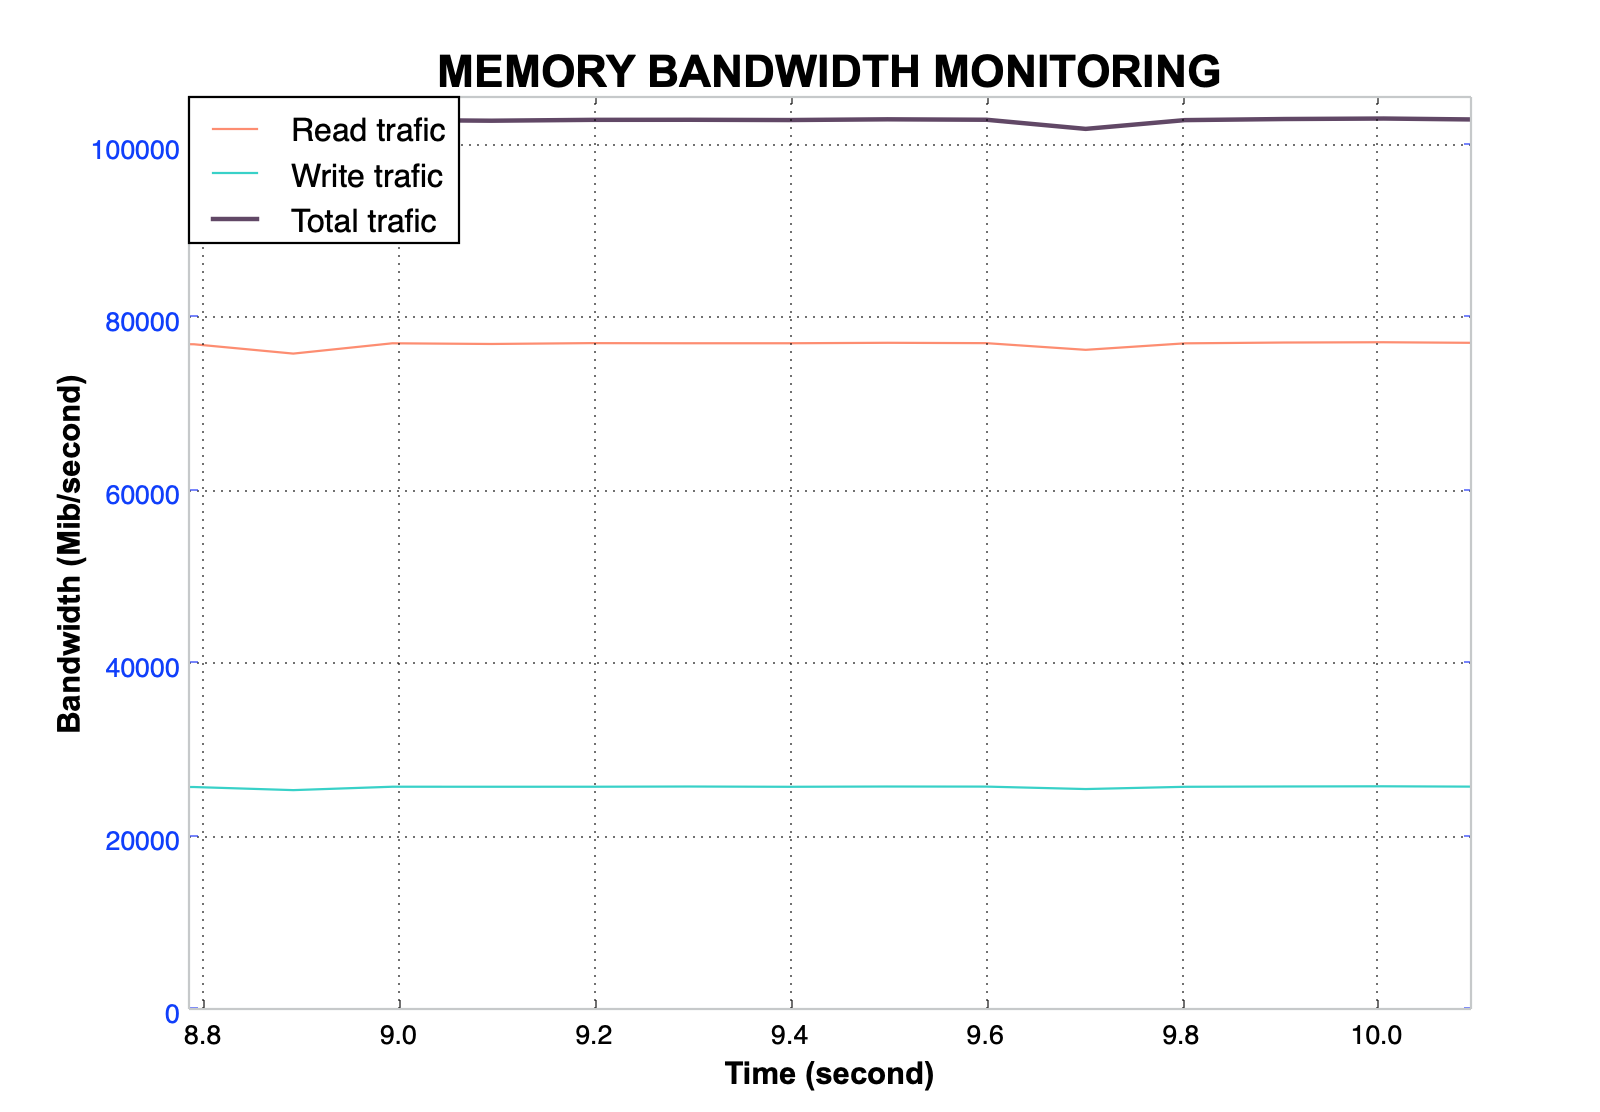
\includegraphics[width=0.80\textwidth]{images/stream_before.png}
        \caption{Prolie mémoire donné par l'outil YAMB pour plusieurs exécution de noyau \textit{triadd} du benchmark \textit{Stream}. }\label{fig:stream_before}
        }
        \end{figure}


        
        \subsubsection{Optimisation du noyau \textit{triadd}}
        %%%%%%%%%%%%%%%%%
            
            Les deux vecteurs B et C doivent nécessairement être lus une fois. La lecture supplémentaire provient du vecteur en écriture. Ce comportement est dû au processeur qui, avant d'écrire une donnée, charge la ligne de cache correspondante pour la mettre à jour. Cependant, le noyau étudié a la particularité d'écrire toute la ligne de cache, les données initialement présentes n'ayant aucune valeur utile. Une option peut être utilisée avec le compilateur Intel (ICC) pour permettre au compilateur d'éviter ce chargement inutile: \verb|-qopt- streaming-stores=always|. Cette option permet au CPU d'écrire toute la ligne de cache sans avoir à la charger.
            
        
        \subsubsection{Performance du noyau optimisé}
        %%%%%%%%%%%%%%%%%
        
            Nous avons compilé \textit{Stream} avec l'option \textit{-qopt- streaming-stores=always} et mesuré le temps et la bande passante de la même manière que pour la première exécution. Les résultats sont résumés dans le \autoref{table:stream_res}. Le temps passé dans le noyau est de 0,59 seconde, beaucoup plus proche du maximum théorique de 0,56 seconde. En analysant la bande passante mémoire, on constate que le rapport lecture/écriture est maintenant de 2 pour 1, les données échangées étant de 34 GB/s en mode écriture pour 68 GB/s en mode lecture. La bande passante total atteint 104 GB/s proche $\text{MEMORY}_{max}$.
            
            %\renewcommand{\arraystretch}{1.2}
            %\setlength{\tabcolsep}{8pt}
            
            \begin{table}[htbp]
            \centering
            \caption{Performance du noyau \textit{triadd} du benchmark \textit{Stream} avant et après optimisation. Le temps (seconde) après optimisation est proche de l'optimum théorique $\text{TEMPS}_{optimal}$  calculé à 0,56 sec. L'utilisation du bus mémoire est approximativement la même entre les deux versions du code (104 et 102 GB/s). L'option de compilation optimise le rapport lecture/écriture (GB/s) et améliore les performances du code de 25\%.}
            \begin{tabular}{l|c|c|c|c|c|}
            \cline{2-6}
            & $\text{TEMPS}_{mesure} (s)$ & Stream   & $\text{YAMB}_{read}$  & $\text{YAMB}_{write}$  & $\text{YAMB}_{total}$  \\ \hline
            \multicolumn{1}{|l|}{Version originale}  & 0.79   & 80.13  & 26        & 78         & 104        \\ \hline
            \multicolumn{1}{|l|}{Version optimisée} & 0.59   & 101.84 & 35        & 69         & 104        \\ \hline
            \end{tabular}
            \label{table:stream_res}
            \end{table}